\documentclass{article}
\usepackage{graphicx}
\usepackage[final]{neurips_2023}
\usepackage[utf8]{inputenc} % allow utf-8 input
\usepackage[T1]{fontenc}    % use 8-bit T1 fonts
\usepackage{hyperref}       % hyperlinks
\usepackage{url}            % simple URL typesetting
\usepackage{booktabs}       % professional-quality tables
\usepackage{amsfonts}       % blackboard math symbols
\usepackage{nicefrac}       % compact symbols for 1/2, etc.
\usepackage{microtype}      % microtypography
\usepackage{xcolor}         % colors
\usepackage{lineno}
\usepackage{amsmath}
\usepackage{float}

\title{Lab 2: CIFAR-10 Image Classification}

\author{
Cuiyang Yong\\
21307140051
}

\begin{document}

\maketitle
% \linenumbers

\begin{abstract}
This report presents an image classification study on the CIFAR-10 dataset using a hierarchical convolutional neural network (CNN) architecture comprising 0.72 million parameters and achieves a test accuracy of 92.51\%, and explores the effectiveness of Batch Normalization (BN) on VCG-A model.\footnote{https://github.com/Snivallus/Neural-Network-Project-2}
\end{abstract}

%=======================================================================
\section{Train a Network on CIFAR-10}

%=======================================================================
\subsection{Methodology}

%=======================================================================
\subsubsection{Data Augmentation}
The CIFAR-10 dataset is a well-established benchmark in the field of machine learning and computer vision, comprised of 60,000 color images, each with a resolution of 32x32 pixels. It is divided into a training set of 50,000 images and a testing set of 10,000 images.

By leveraging PyTorch’s \textbf{torchvision} library, this report applies data augmentation techniques to increase variability in the training data. Each training sample undergoes the following transformations:

\begin{itemize}

    \item \textbf{Normalization:} Each image is normalized using the CIFAR-10 training set mean (0.4914, 0.4822, 0.4465) and standard deviation (0.2470, 0.2435, 0.2616).

    \item \textbf{Random Cropping:} This process involves randomly selecting a subregion of the image and rescaling it to the original dimensions.

    \item \textbf{Horizontal Flipping:} Images are randomly mirrored along the vertical axis.

    \item \textbf{Color Jittering:} Adjusts the brightness, contrast, saturation, and hue of images randomly.
    
\end{itemize}

%=======================================================================
\subsubsection{Model Structure}

The \textbf{Basic Block} is a modular convolutional unit designed for flexible feature extraction and channel attention. Internally, it stacks multiple convolutional layers, each composed of a 2D convolution, batch normalization, and an activation function, followed by an optional residual downsample branch if required. The output of the convolutional sequence is added to the appropriate identity pathway—either the original input or a downsampled version—forming a standard residual connection, after which a Squeeze-and-Excitation (SE) module is applied to boost representational power.

The overall architecture begins with a "stem" convolution that maps the three-channel CIFAR-10 input to $24$ feature channels. Concretely, the stem consists of a $5\times 5$ convolution, followed by BatchNorm and the chosen activation function (ReLU, Sigmoid, or Tanh). The subsequent feature extractor is divided into three stages, each comprised of $7$ instances of the basic block.

\begin{itemize}
    \item Stage $1$ retains a constant channel width of $24$ throughout, without any downsampling.

    \item Stage $2$ increases the channel width from $24$ to $32$, with downsampling in the first block.

    \item Stage $3$ raises the channel width from $32$ to $64$, with downsampling in the first block.
\end{itemize}

After these three stages, each $64$-channel feature is flattened by an adaptive average pooling layer, then passed through a fully connected layer mapping $64$ inputs to $128$ units, followed by the same activation, a Dropout($0.5$), and a final linear classifier producing $10$ logits. 

All convolutional and linear layers are initialized via Kaiming Normal (for ReLU) or Xavier Uniform (for Sigmoid/Tanh), with BatchNorm weights set to $1$ and biases to $0$.

%=======================================================================
\subsubsection{Training Procedure}

The network is trained for a fixed number of epochs on CIFAR-10, using the Adam optimizer and an adaptive learning‐rate schedule with a warmup phase. The custom scheduler gradually increases the learning rate from near zero to the preset maximum over a small number of “warmup” epochs; once warmup is complete, the schedule holds the learning rate constant before entering a cosine‐decay phase over the remaining epochs.

During each epoch, the training set is iterated in randomized batches. For every batch, the model performs a forward pass to compute the loss and accuracy, followed by a backward pass to accumulate gradients. Optionally, gradient norms are clipped after warmup to prevent exploding gradients. The optimizer then updates model parameters using the computed gradients. An early‐stopping monitor tracks validation accuracy: if no improvement exceeding a small threshold is observed for a preconfigured number of consecutive epochs, training halts prematurely.

%=============================================================
\subsection{Experiments}

%=============================================================
\subsubsection{Insights}

The proposed model was trained using a subset of 10,000 samples from the CIFAR-10 training set, where each image was subjected to two independent transformations for data augmentation.

\begin{table}[H]
  \centering
  \caption{Hyperparameter settings}
  \label{tab:model_setting}
  \begin{tabular}{cc}
    \toprule
    \textbf{Hyperparameters} & \textbf{Settings} \\
    \midrule
    \textbf{Batch Size} &\\
    Train Batch Size & 256\\
    Test Batch Size & 512\\
    \midrule
    \textbf{Data Augmentation} &\\
    Random Crop & padding=4, padding\_mode= reflect \\
    Color Jitter & brightness=0.3, contrast=0.3, saturation=0.3, hue=0.15 \\
    Normalization & mean=(0.4914, 0.4822, 0.4465), std=(0.2470, 0.2435, 0.2616)\\
    \midrule
    \textbf{Loss Function} & Cross-Entropy \\
    \midrule
    \textbf{Activation Function} & ReLU\\
    Weight Initialization & Kaming Normal\\
    Dropout & Normal Dropout \\
    Dropout Rate & 50\%\\
    \midrule
    \textbf{Optimizer} & Adam \\
    Max Learning Rate & 0.0006\\
    Weight Decay & 0.0002\\
    Gradient Clip & 1.0\\
    \midrule
    \textbf{Early Stopping} &\\
    Patience & 20 \\
    Min Delta & 0.001\\
    \midrule
    \textbf{Model Metrics}\\
    Params (M) & 0.72\\
    Params Size (MB) & 2.75\\
    Forward/Backward Pass Size (MB) & 14.55\\
    Total Size (MB) & 17.31\\
    GFLOPs & 0.143\\
    \bottomrule
  \end{tabular}
\end{table}

 Under this training regime, the model achieved a classification accuracy of 92.51\% on the test set. The full hyperparameter configuration and resource metrics are summarized in Table \ref{tab:model_setting}.

We selected the $24$ filters of the first convolutional layer and arranged them in a $4\times 6$ grid for compact representation. To ensure interpretability, each filter was normalized independently to the $[0, 1]$ range and mapped to grayscale intensities. It is observed that many filters exhibit localized edge-detecting behavior, with strong horizontal, vertical, or diagonal orientations. Others capture color contrast patterns or blob-like structures that are indicative of primitive shape detection.

\begin{figure}[H]
  \centering
  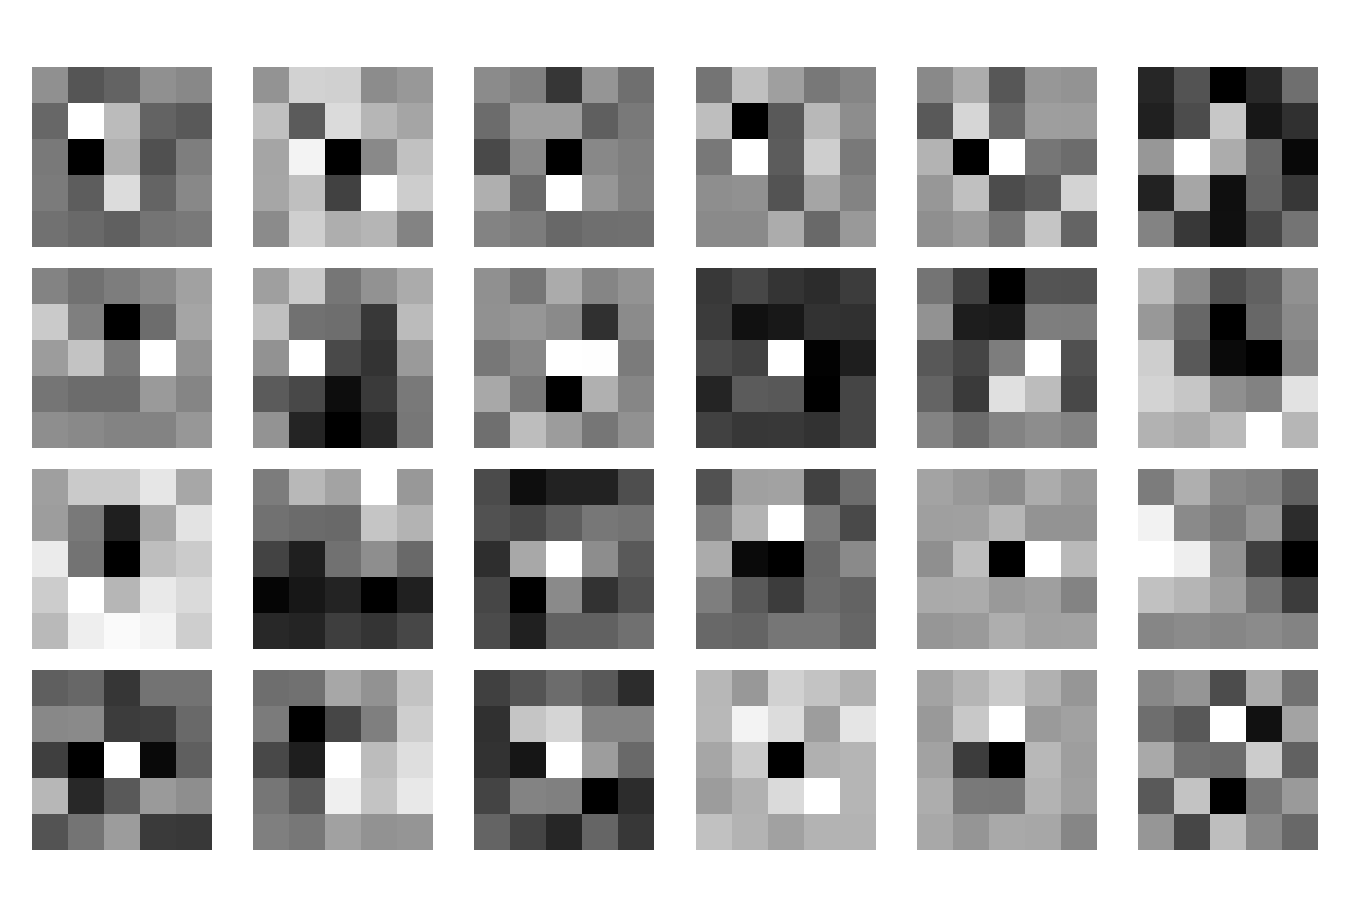
\includegraphics[width=0.8\linewidth]{figures/filter_visualization.pdf}
  \caption{Visualization of the first-layer convolutional filters (grayscale).}
  \label{fig:first_layer_filters}
\end{figure}

The loss landscape shown in figure\ref{fig:loss_landscape} illustrates the topography of the model's objective function in a projected subspace of the high-dimensional parameter space.

\begin{figure}[H]
  \centering
  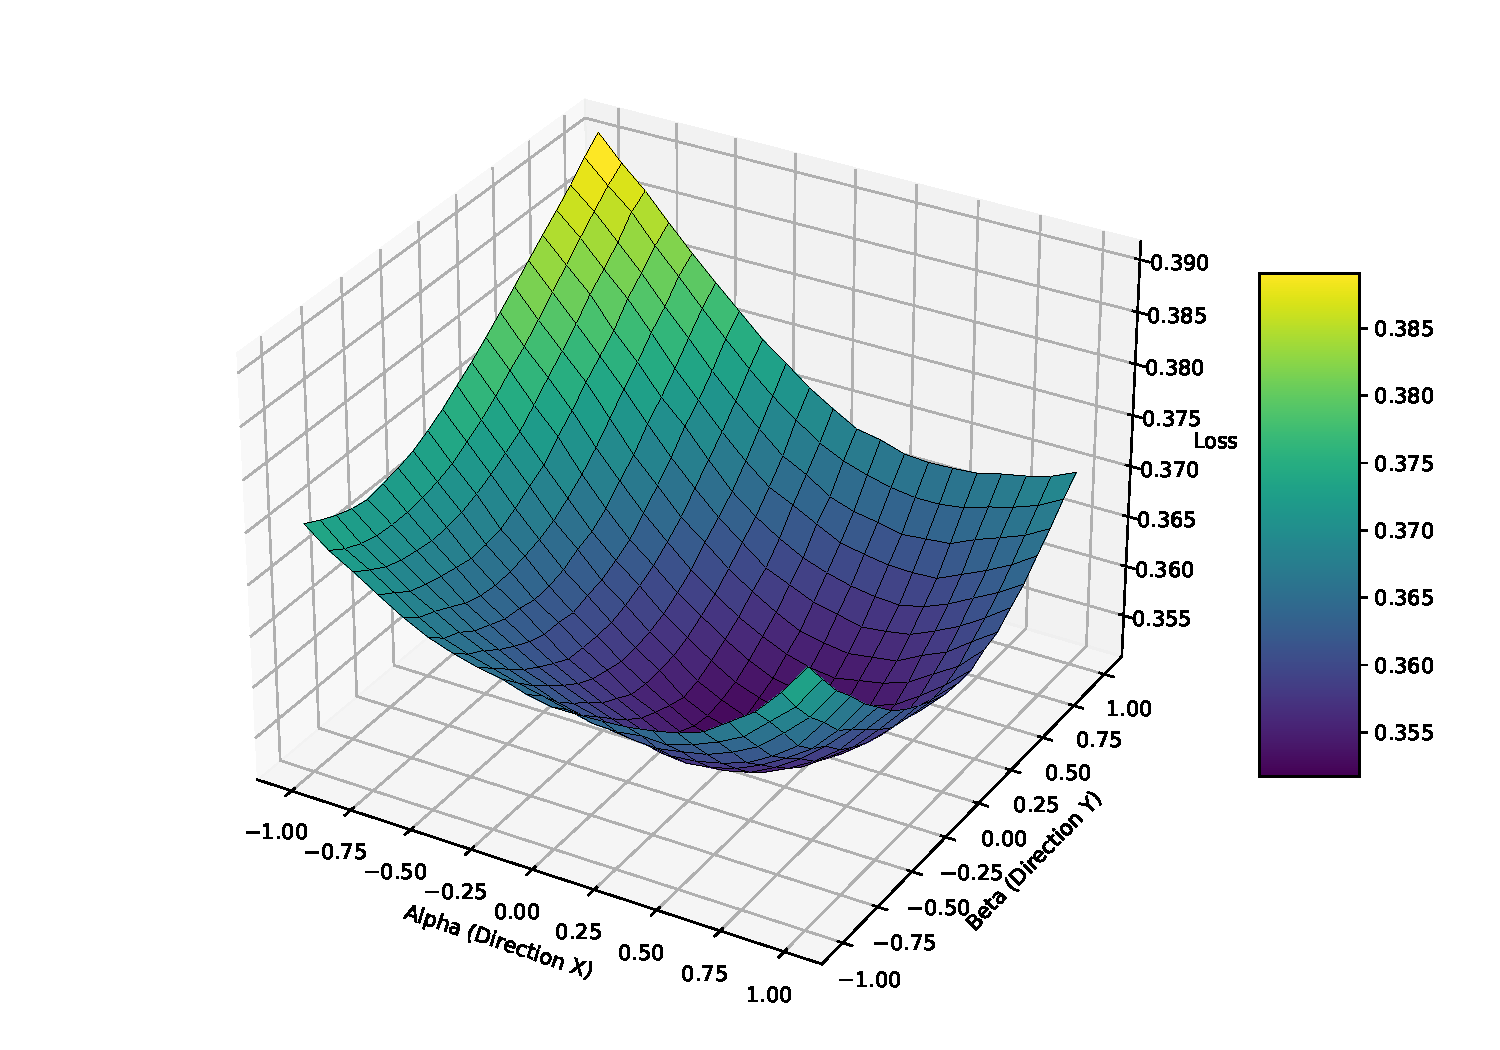
\includegraphics[width=0.8\linewidth]{figures/loss_landscape_3d.pdf}
  \caption{Loss landscape.}
  \label{fig:loss_landscape}
\end{figure}

%=============================================================
\subsubsection{Different Activation}

The results of training the same model architecture with different activation functions (ReLU, Tanh, and Sigmoid) under identical conditions demonstrate a clear hierarchy in effectiveness: ReLU outperforms Tanh, while Sigmoid consistently underperforms both——likely due to its susceptibility to the vanishing gradient problem.

\begin{figure}[H]
  \centering
  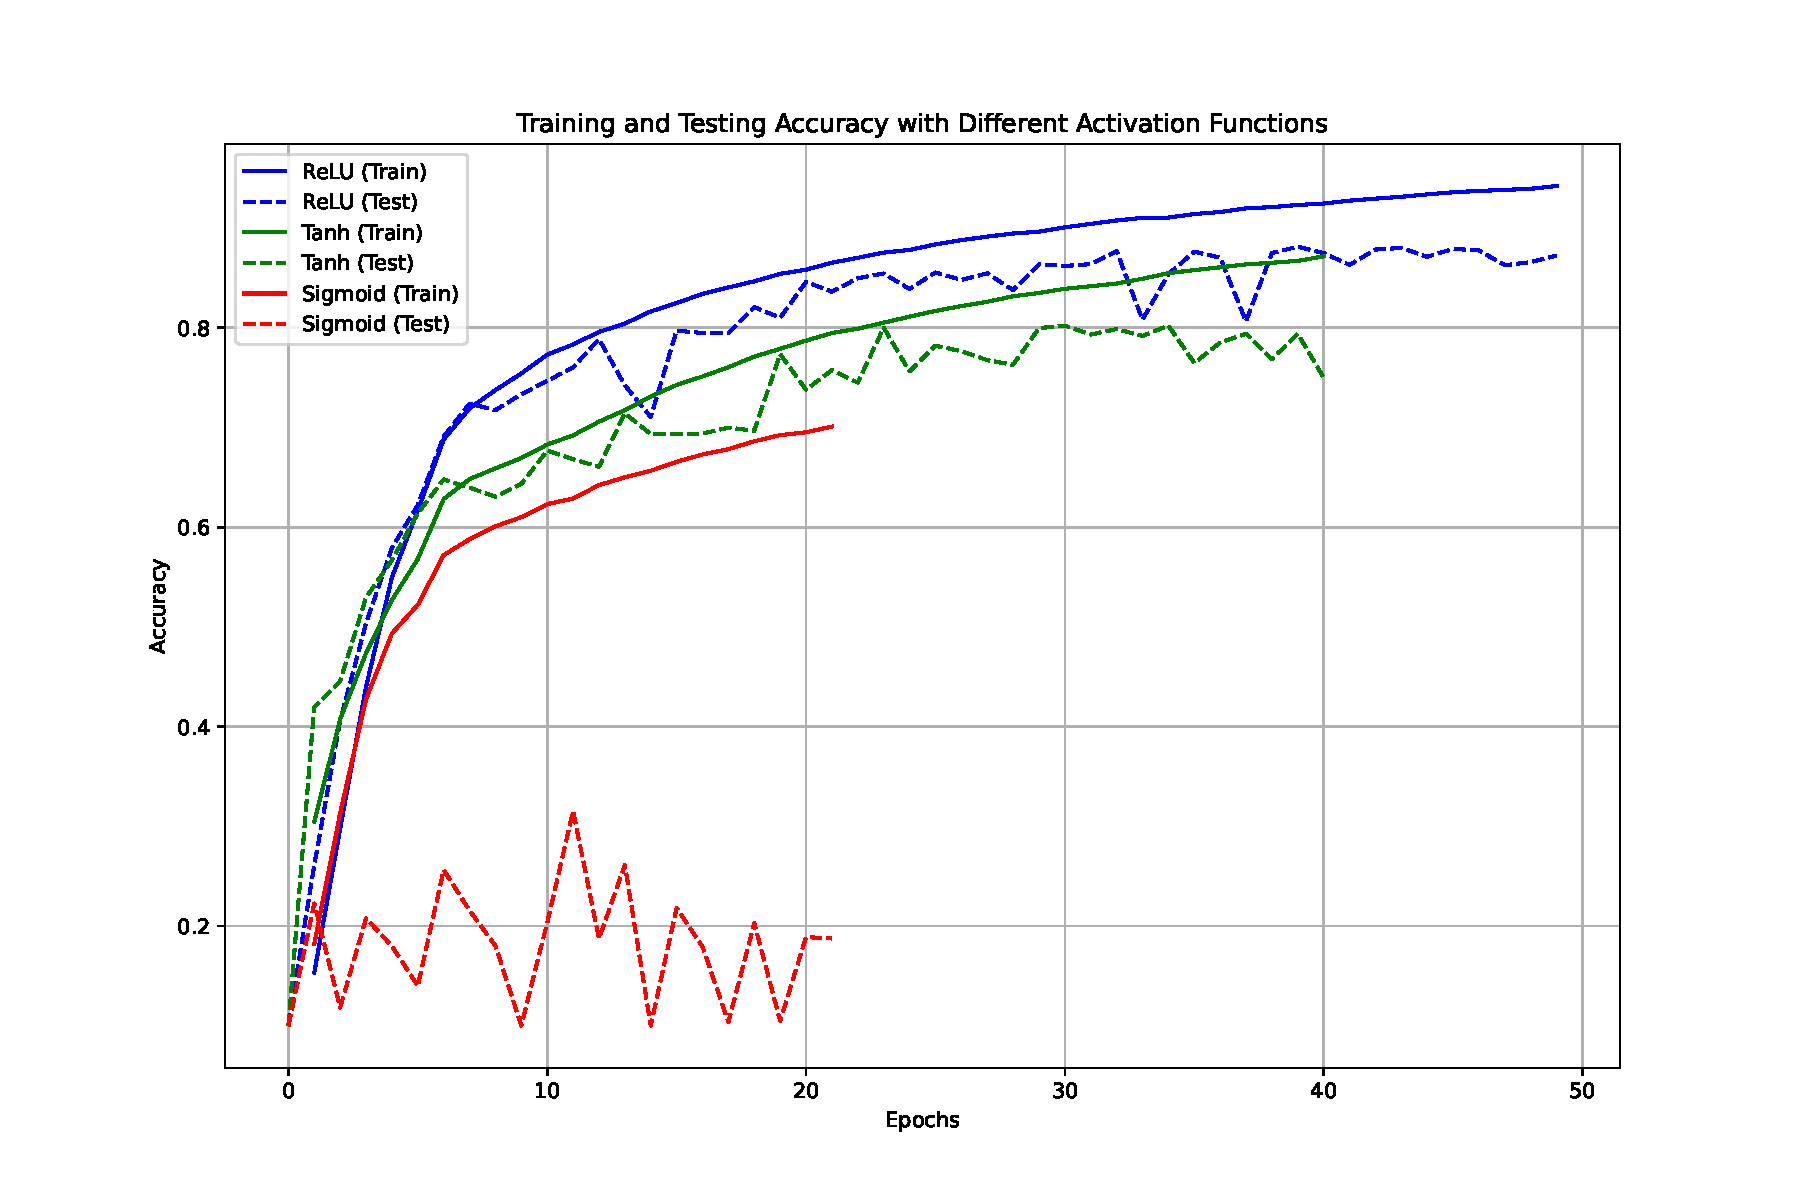
\includegraphics[width=0.7\linewidth]{figures/accuracy_different_activation.pdf}
  \caption{Accuracy with different activation functions.}
  \label{fig:accuracy_different_activation}
\end{figure}

%=============================================================
\subsubsection{Different Structure}

The results of training the same model architecture with varying numbers of convolutional blocks in each stage reveal a significant influence of network depth and structural complexity on performance.

\begin{figure}[H]
  \centering
  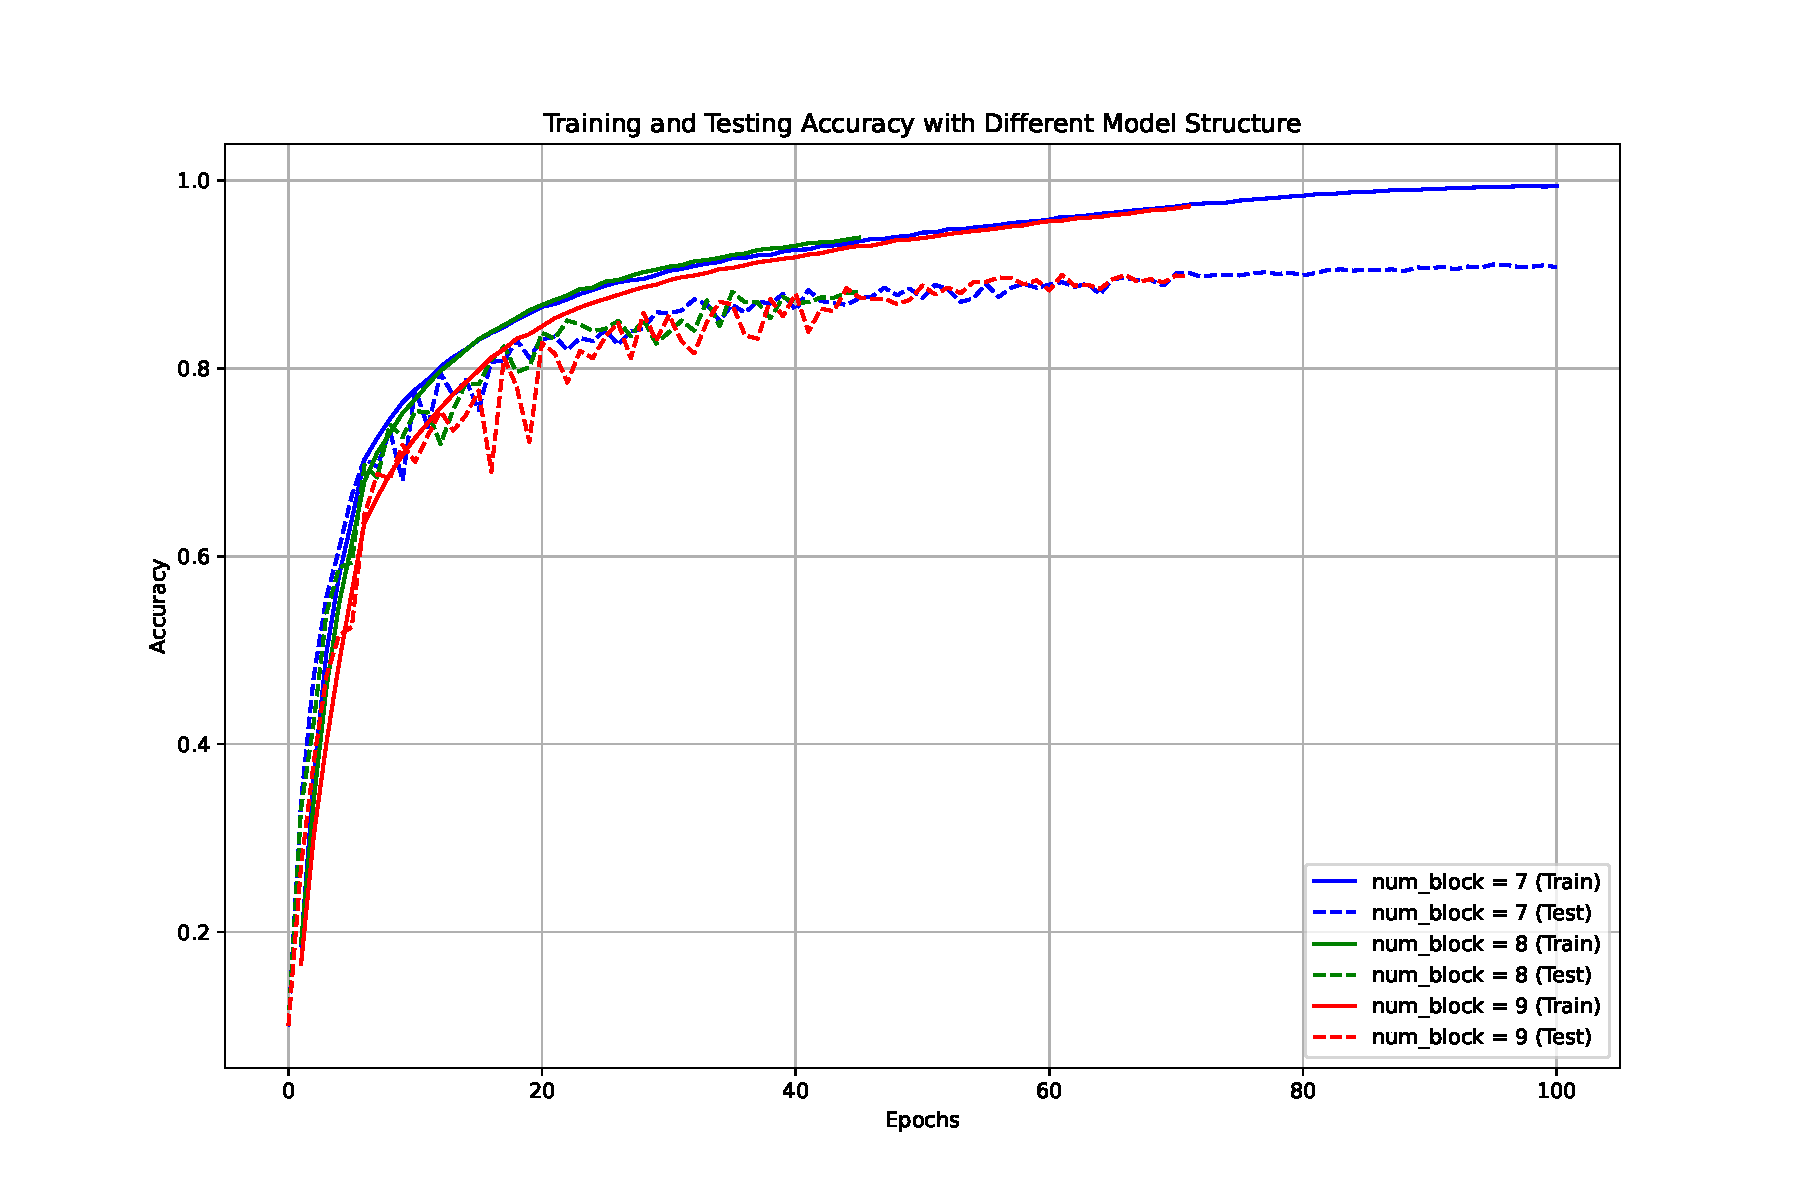
\includegraphics[width=0.7\linewidth]{figures/accuracy_different_structure.pdf}
  \caption{Accuracy with different structure.}
  \label{fig:accuracy_different_structure}
\end{figure}

We observed that adding a reasonable number of blocks per stage improves both convergence speed and final accuracy. However, beyond a certain threshold, the performance gains taper off or even degrade slightly. 

%=============================================================
\subsubsection{Different Loss}

The results of training the same model architecture under identical conditions but with varying values of weight decay are as follows: 

\begin{figure}[H]
  \centering
  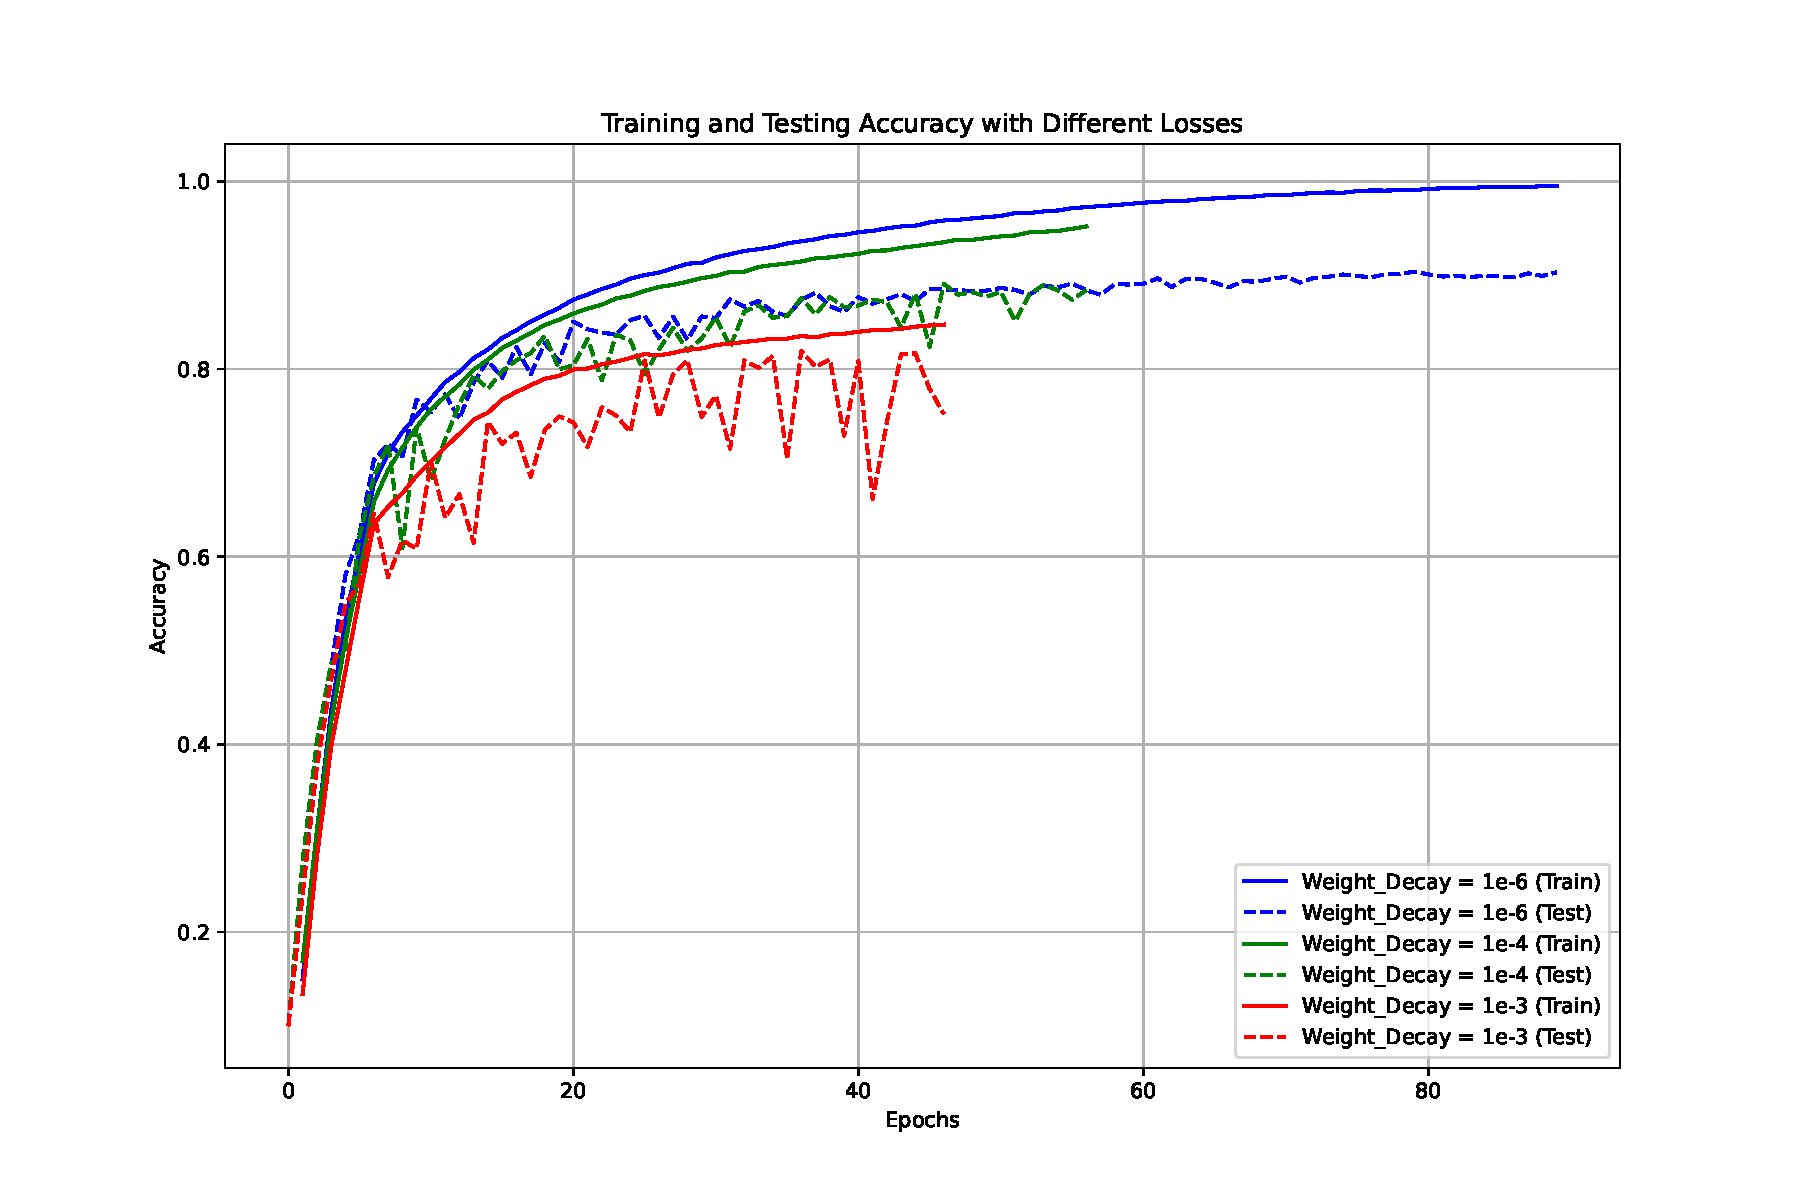
\includegraphics[width=0.7\linewidth]{figures/accuracy_different_loss.pdf}
  \caption{Accuracy with different loss.}
  \label{fig:accuracy_different_loss}
\end{figure}

Moderate weight decay helped control the magnitude of the weights, leading to smoother and more robust decision boundaries.
However, when the weight decay value was set too high, the performance began to deteriorate, that is, the model underfits the data, failing to capture important patterns even in the training set.

%=============================================================
\subsubsection{Different Optimizer}

The results of training the same model architecture under identical conditions but with different optimizers—namely Stochastic Gradient Descent (SGD) and Adam—highlight fundamental differences in optimization dynamics and their impact on convergence speed and generalization performance.

\begin{figure}[H]
  \centering
  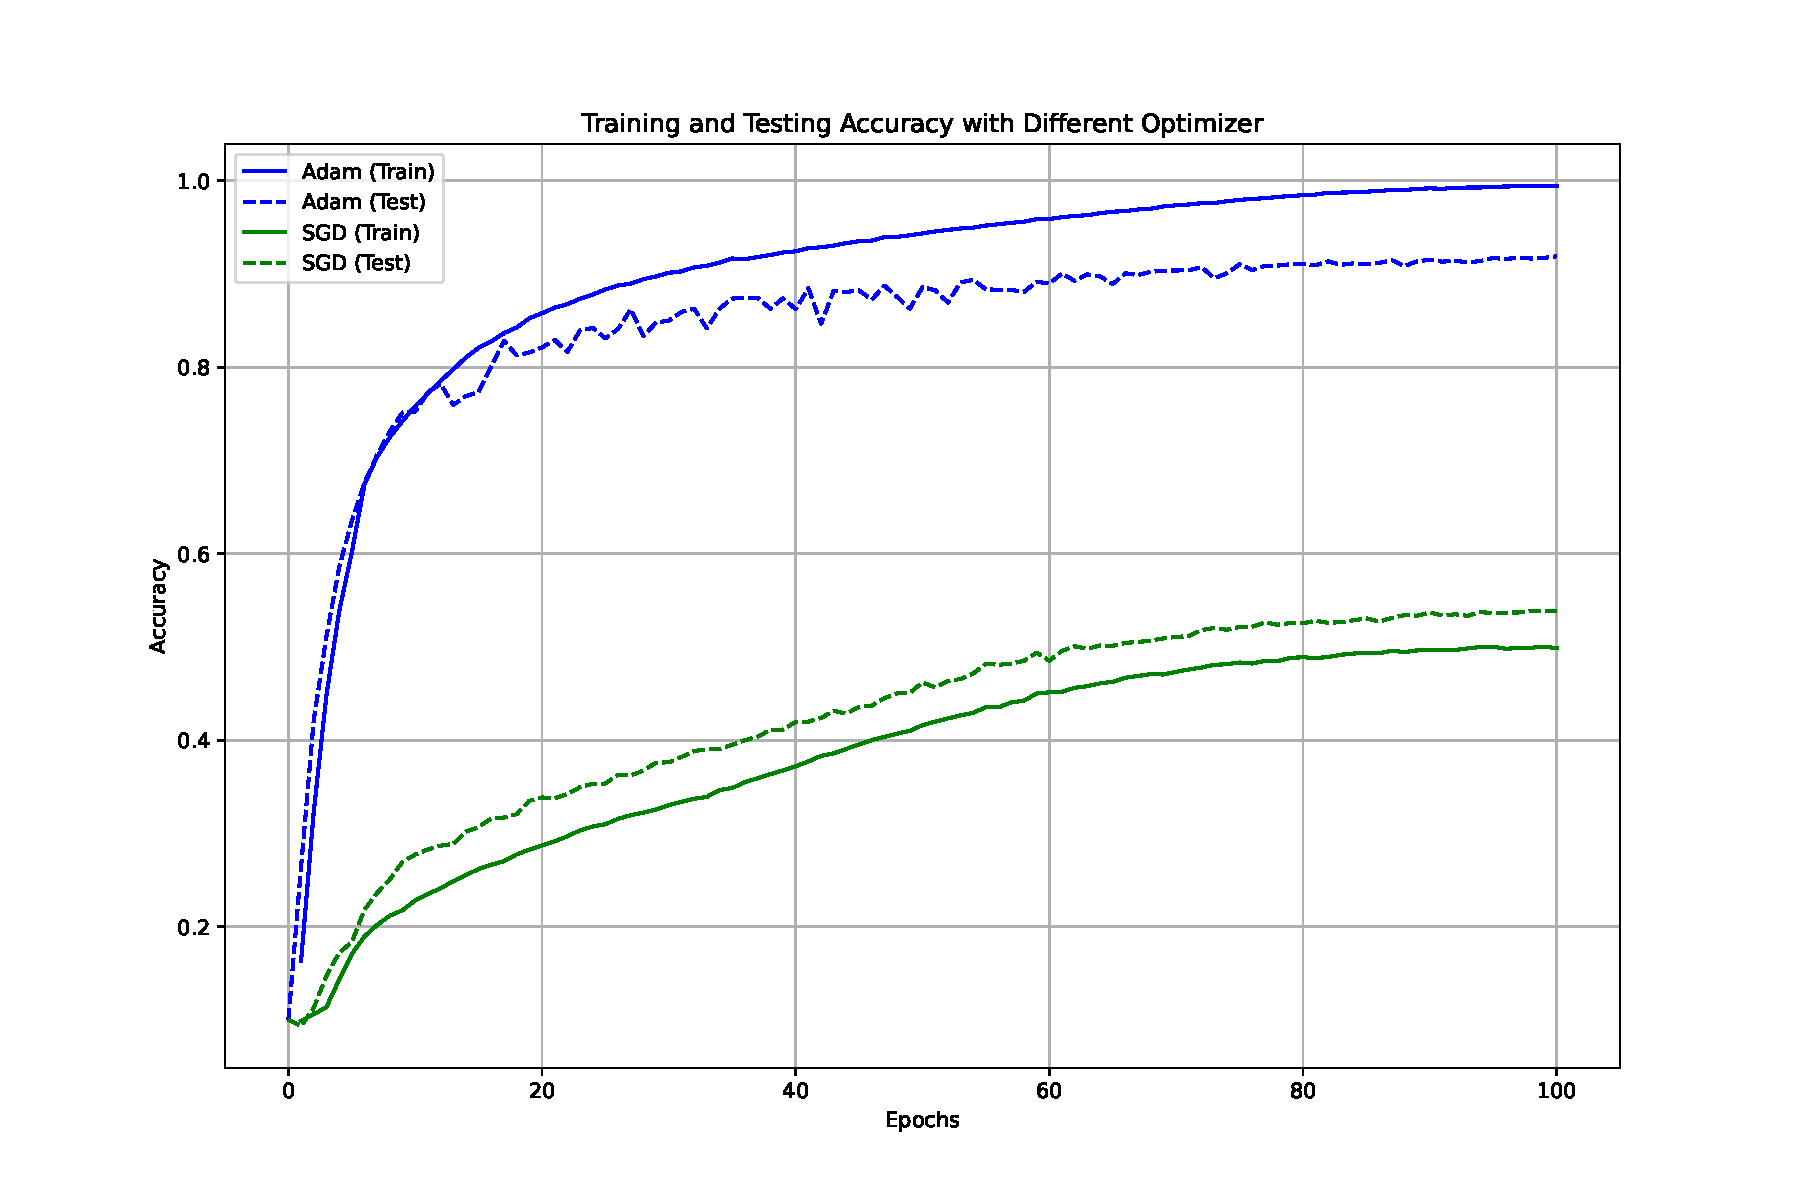
\includegraphics[width=0.7\linewidth]{figures/accuracy_different_optimizer.pdf}
  \caption{Accuracy with different optimizer.}
  \label{fig:accuracy_different_optimizer}
\end{figure}

It is observed that Adam converges significantly faster than SGD in the early stages of training. This rapid progress is attributed to its adaptive learning rate mechanism, which is especially effective in handling sparse gradients or varying curvature across dimensions.

\section{Batch Normalization}

Batch Normalization (BN) normalizes data within the same batch across each dimension, while also supporting scale and shift transformations, which stabilizes the distribution of intermediate layers. In practice, BN has been shown to significantly impact model optimization and final performance. In this experiment, based on the VGG-A architecture, we compare the training performance of models with and without batch normalization. We implemented VCG-A with BN (\texttt{VGG\_A\_BatchNorm}) in \texttt{vgg.py} by adding a \texttt{BatchNorm2d} layer after each convolutional layer. Then, we trained both versions of the VGG-A model on the CIFAR-10 dataset using different learning rates. The experimental parameter settings are shown in the table below.

\begin{table}[H]
\centering
\caption{VGG-A Comparision Setting}
\label{tab:vgg_bn_settings}
\begin{tabular}{cc}
\toprule
\textbf{Hyperparameters} & \textbf{setting} \\
\midrule
Optimizer & Adam \\
Loss Function & Cross-Entropy \\
Batch Size & 128 \\
Epoches & 20 \\
\bottomrule
\end{tabular}
\end{table}

\subsection{Training Process Comparison}

We trained the VGG-A models with and without Batch Normalization (BN) using learning rates of $0.0005$ and $0.001$, respectively.

\begin{table}[H]
    \centering
    \caption{VGG-A training process comparison}
    \label{tab:vgg_bn_results}
    \begin{tabular}{ccc}
        \toprule
        \textbf{Model} & \textbf{Learning Rate} & \textbf{Test Accuracy} \\
        \midrule
        VGG-A & 0.0005 & 84.84\% \\
        VGG-A-BN & 0.0005 & 86.66\% \\
        \midrule
        VGG-A & 0.001 & 82.44\% \\
        VGG-A-BN & 0.001 & 86.96\% \\
        \bottomrule
    \end{tabular}
\end{table}

The model with Batch Normalization (BN) achieves significantly higher accuracy on the validation set, indicating that BN facilitates optimization to some extent. 

\subsection{Loss landscape Comparison}

To visualize the loss landscape, we generate an intuitive 2D representation that captures how loss values evolve during training across different model instances and hyperparameters. This involves training multiple versions of a model (e.g., VGG variants) with varied learning rates to explore diverse optimization trajectories. 

At each training step (typically every batch), we collect the loss values from all model instances, compute the minimum and maximum losses, and form boundary curves. The area between these curves is then filled to create a band in the plot—where the x-axis represents training steps and the y-axis represents loss. This band illustrates the range of loss behaviors for a given architecture, with its width indicating sensitivity to hyperparameters, height reflecting absolute loss levels, and slope revealing convergence speed. 

\begin{figure}[H]
  \centering
  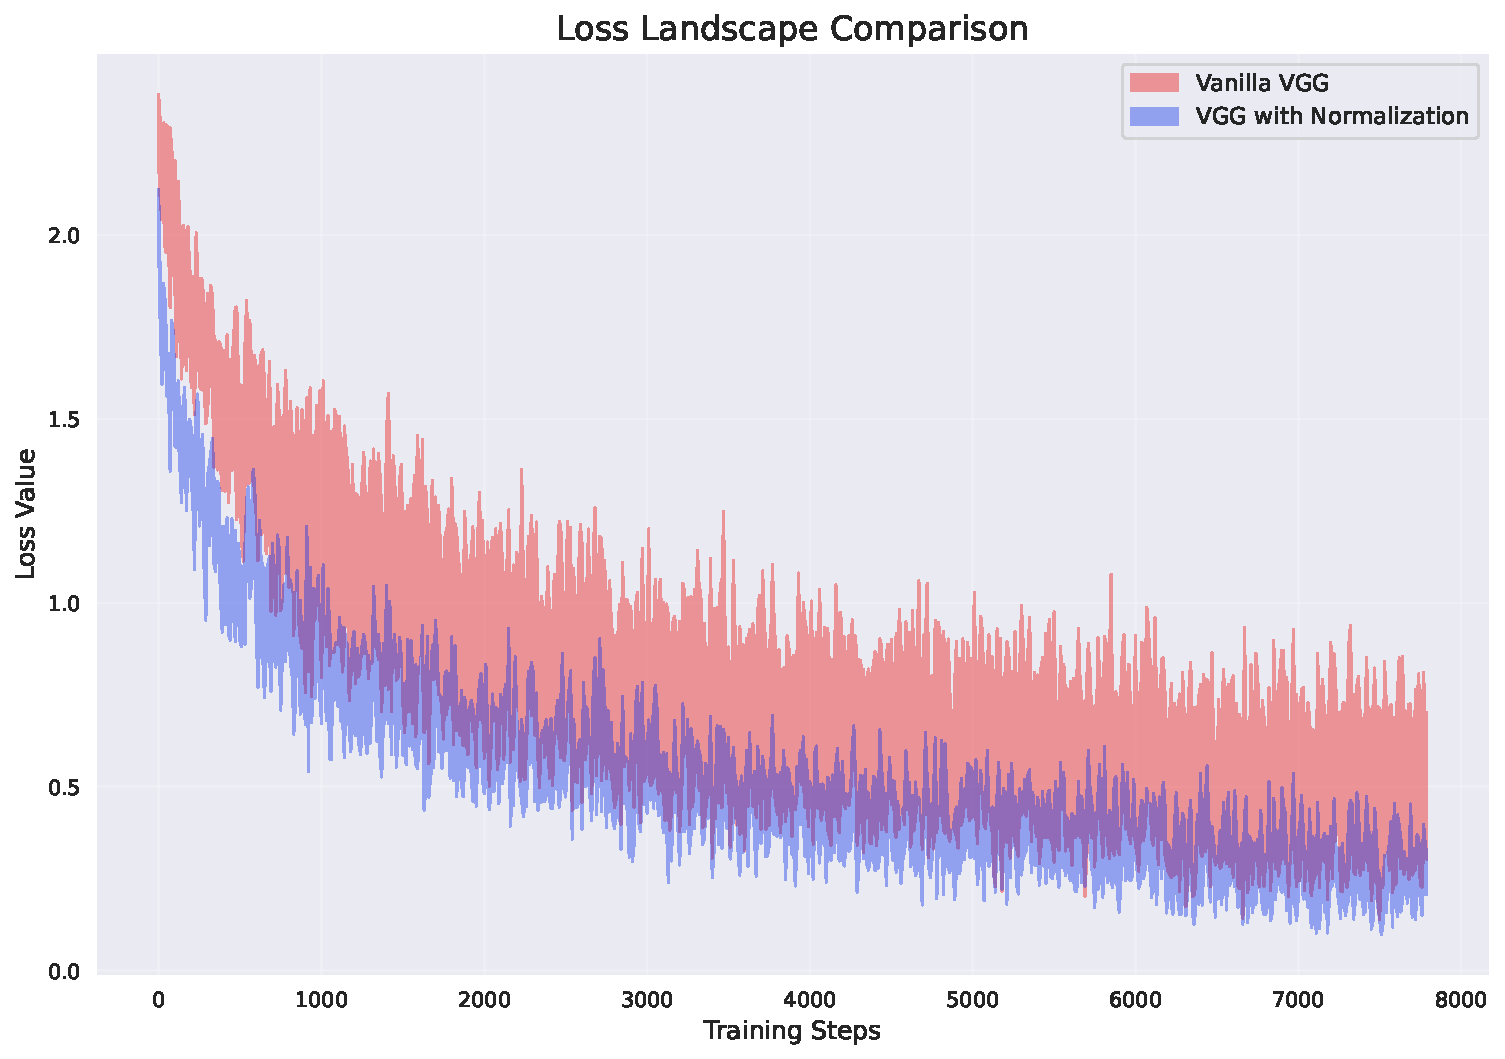
\includegraphics[width=0.8\linewidth]{figures/landscape_comparison.pdf}
  \caption{Loss landscape Comparison.}
  \label{fig:landscape_comparison}
\end{figure}

\end{document}